\documentclass[11pt]{article}

\usepackage[margin=2.3cm]{geometry}
\usepackage{graphicx}
\usepackage{amsmath,amssymb}
\usepackage{booktabs}
\usepackage{siunitx}
\usepackage{microtype}
\usepackage[hidelinks]{hyperref}
\usepackage{caption}
\captionsetup{font=small,labelfont=bf}
\graphicspath{{jerry_figures/}}

\setlength{\columnsep}{0.7cm}

\title{\vspace{-1.2em}\textbf{Frequency-Multiplexed Closed-Loop Control of a\\
Brain--Machine Hand Interface}}
\author{GG4 --- Neural Data Analysis with Adaptive State Estimation \\
\texttt{yhl63} (Jerry Liu)}
\date{\vspace{-0.8em}}

\begin{document}
\maketitle

\begin{abstract}
\noindent
I drive a simulated hand to Cartesian targets by commanding a two-dimensional
stimulation of a stochastic ``brain'' whose noisy 16-D activity passes through a
fixed, stateful, nonlinear decoder before moving a two-link arm. The end-to-end
map is nonlinear, partially observable, non-invertible and noisy, so no standard
linear controller applies directly. The contribution is a control \emph{abstraction}
obtained by reverse-engineering the decoder: it is a \emph{frequency-addressed
muscle bank}, and a small sinusoidal ``select tone'' at a muscle's frequency,
exploiting the fact that the head's power channel is held on ``for free'' by a
latent DC offset, drives that muscle. This reduces control to two independent
inverse-kinematics joint servos closed on the hand position. The controller
reaches the upper, well-actuated half of the workspace to within
$\sim$6\,cm and generalises across brains (median 10\,cm, 93\% within 15\,cm), but
the brain's low-pass character makes the high-frequency (elbow) muscles weak,
producing a sharp, directionally-structured failure in the lower workspace. I
quantify this, contrast a hand-feedback (V1) and a neural-observer (V2) variant to
measure the value of sensing ($\sim$24\,cm), and show the binding precision limit
is a property of the plant, not the control law.
\end{abstract}

\section{Introduction}
The GG4 platform poses two coupled problems: \emph{estimation} --- recovering
hidden structure from noisy neural observations --- and \emph{control} ---
commanding inputs to produce a desired behaviour. This report concerns the final
control task: steering a hand to a target $(x,y)$ using only the official
interface, namely the per-step neural measurement \texttt{measure()}, the current
hand position \texttt{hand\_pos}, and the input \texttt{next\_state(u)} with
$u\in[0,1]^2$.

The plant is a composition:
\[
\resizebox{\linewidth}{!}{$\displaystyle
u \to \underbrace{\text{brain}}_{\text{LGSSM, random}} \to \text{neural} \to
\underbrace{\text{decoder}}_{(x_1,x_2)} \to \underbrace{\text{head}}_{\text{nonlinear}}
\to \text{4 muscles} \to \text{arm} \to \text{hand}.$}
\]
It is nonlinear, partially observable, non-invertible and stochastic, and the hard
part is not any single stage but the \emph{interface} between a linear,
identifiable front end (the brain) and a nonlinear, rhythm-coded back end. The
first half of the work was therefore reverse-engineering the plant until a control
abstraction emerged; the second half was a controller built on it and its honest
evaluation. The full design log is given in the accompanying lab notebook.

\section{Plant structure and key findings}
\label{sec:plant}
I treat the per-trial \emph{brain} as unknown but identifiable, and the
\emph{decoder + head + arm} as a \emph{fixed, brain-invariant} apparatus,
identical on every trial. This split is the central structural lever: the random
part of the plant is the easy linear part, and the hard nonlinear part never
changes. The following were established empirically; several required an exact
NumPy replica of the head, verified to match the supplied Torch network to
$3\times10^{-7}$ and used as a glass-box to read its hidden internal state.

\paragraph{Frequency-addressed selection.} The decoder is linear,
$(x_1,x_2)=D\,y+b$. A bank of cosine/sine band-pass filters acts on the recent
history of $x_1$; each of the four muscles responds to a distinct frequency
($\approx0.073,0.133,0.207,0.312$ cycles/sample). Driving $x_1$ to oscillate near
a muscle's frequency selects it, and the selector saturates easily, so
\emph{selection is the easy half}.

\paragraph{Power is ``free''.} The head enables a muscle only when $x_2$ clears a
wake threshold ($\approx+0.72$) with persistent evidence. Crucially, $x_2$ sits at
a large positive DC offset ($\approx+1.8$) under neutral input that already
exceeds threshold, and the head's evidence rule (the ``same-sign-a-period-apart''
weight $0.30$ exceeds the evidence threshold $0.16$) means a \emph{constant-high}
$x_2$ sustains power indefinitely: feeding the replica a constant $x_2=1.5$ holds
power at $0.654\pm0.00$. We therefore never synthesise a power signal; we only
avoid letting $x_2$ dip below threshold.

\paragraph{Velocity, not position.} Muscle activation is $\text{power}\times
\text{selector}\in[0,1]$; the arm converts antagonist differences into joint
angular \emph{velocity} through dry-(stiction) and wet-(viscous) friction. Hand
position is thus the time-integral of a velocity we modulate, and below the
stiction threshold the joint \emph{holds} --- a free brake.

\paragraph{Low-pass, noisy brain.} Because the brain is an approximately LTI
state-space system, a tone at frequency $f$ in $u$ produces latent oscillation at
the same $f$, with amplitude and phase set by the brain's transfer function
$G(f)$. System identification (\S\ref{sec:estimation}) shows $G$ is low-pass: the
spectral radius is $\rho(A)\approx0.9$--$0.95$ and the input--output coherence
collapses above $\sim0.1$\,cyc/sample. Consequently the higher-frequency muscles
receive less drive and are weaker --- the single fact behind the controller's
dominant failure mode. Finally, a single \texttt{measure()} is very noisy
($\sigma\approx2.6$); the arm is driven by a 100-sample average ($\sigma\approx
0.25$), but the controller sees only the single sample, so the loop must be closed
and evaluation must be multi-trial.

\section{Estimation: brain identification and the hand observer}
\label{sec:estimation}
Estimation enters the control pipeline in three places, reusing the
linear-Gaussian state-space machinery developed earlier in the project.

\paragraph{Brain system identification.} Driving the brain with a
persistently-exciting bounded probe and fitting an LGSSM by
expectation--maximisation (with a subspace warm start) yields
$(A,B,C,Q,R)$. The identified model's frequency response, compared against an
empirical transfer function measured by a periodic multisine
(Fig.~\ref{fig:frf}), characterises the brain: its dominant principal gain falls
roughly an order of magnitude across the band, so it is open-loop stable and
low-pass --- exactly what motivates and explains the muscle-strength asymmetry of
\S\ref{sec:plant}. Identification is well posed here because, unlike the blind
setting of the earlier estimation weeks, the inputs are known.

\begin{figure}[t]
\centering
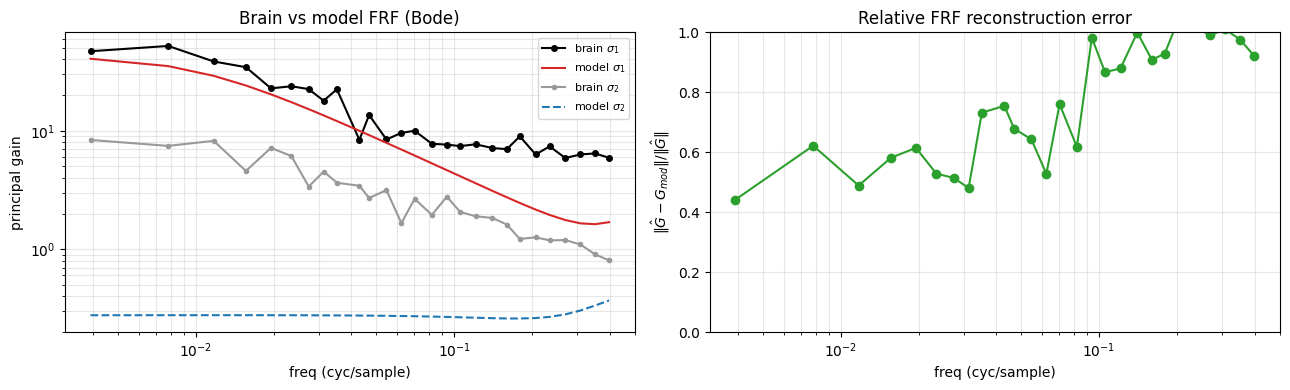
\includegraphics[width=\linewidth]{brain_frf.png}
\caption{Brain frequency response. Left: measured (black/grey) vs.\ identified-model
(red/blue) principal gains. The dominant gain $\sigma_1$ rolls off from $\sim$40 to
$\sim$6 with frequency --- a direct measurement of the low-pass character that
makes the high-frequency (elbow) muscles weak. Right: the model's relative
reconstruction error grows with frequency, where the brain transmits little and
coherence is lost.}
\label{fig:frf}
\end{figure}

\paragraph{Latent decoding.} Because the decoder $D$ is fixed and known, the
control-relevant latents $(x_1,x_2)=Dy+b$ are computable from the neural
observations even though the head exposes only muscle outputs. This is what allows
the glass-box analysis and the input-design reasoning.

\paragraph{Hand-state estimation.} The controller needs the joint state. In V1
this is read directly from the measured hand position by inverse kinematics. In V2
it is produced by a forward observer that replays the fixed downstream
(decoder$\to$head$\to$arm-velocity) on the observed neural and integrates a
joint-angle estimate, using no hand feedback. The two variants are precisely a
Kalman \emph{predict-plus-update} versus a \emph{predict-only} estimator applied
to the hand, and their gap (\S\ref{sec:results}) measures the value of the hand
measurement.

\section{Control approach}
\label{sec:control}

\subsection{Why standard linear control does not transfer}
LQG regulates a linear state to a \emph{static} setpoint, but the hand is not in
the brain's state (there is no arm$\to$brain feedback) and the head needs
\emph{oscillation} to move at all --- the opposite of settling to a constant.
Feed-forward Fourier/SVD inversion of the brain can synthesise any reachable
\emph{latent} trajectory, but cannot cross the nonlinearity to a position
reference and has no mechanism to correct the integrator under noise. Nonlinear
MPC could in principle target the hand but requires a full model of the unknown,
stochastic stack and a non-convex solve. The conclusion is structural: linear
tools belong on the inner channel (produce the right latent oscillation), and the
outer problem (position, through a nonlinear integrator) must be closed with
feedback on an estimated velocity.

\subsection{Design ladder: how the controller was found}
The final controller is the end of a short ladder of designs, each discarded for a
specific, observable reason --- a process worth recording because it justifies the
final form rather than asserting it. \emph{(i) Naive two-tone.} Following the
literal description of the head, drive $x_1$ with a select tone and $x_2$ with a
slow power tone. This fails: the select tone, transported into both latents,
contaminates $x_2$, which dips through the wake threshold; because the head's power
exits fast but re-enters slowly, each dip crashes power and it recovers only
slowly, giving a single ``fire-once'' slew followed by an un-retriggerable
latch-off. \emph{(ii) Clean separation by input-direction nulling.} The principled
fix uses the two channels to drive $x_1$ while \emph{nulling} $x_2$ at the select
frequency --- a well-conditioned $2\times2$ solve. The selection nulling works, but
the full scheme also requires a clean, centred $x_2$ power oscillation, and
centring the large $+1.8$ offset consumes nearly all of the $[0,1]$ headroom, so
the select tone clips and clipping re-introduces the contamination; moreover,
measuring the per-frequency response online costs $\sim$1500 steps, over the
400-step budget. \emph{(iii) Power from the offset.} The breakthrough
(\S\ref{sec:plant}) dissolves the problem: $x_2$'s natural offset already holds
power on, so the power tone and the centring are dropped entirely, and the only
remaining job --- a small select tone --- is so small that $x_2$ never dips, making
the nulling unnecessary too. The result is the simple, affordable, single-direction
drive used below.

\subsection{The select-tone joint servo (V1)}
The design exploits the structure of \S\ref{sec:plant} directly.

\emph{Inner channel.} To fire a muscle I drive a sinusoidal select tone at its
frequency; power comes free from the $x_2$ offset, so no power tone and no
DC-centring are needed. The tone amplitude is kept small enough that its
inevitable leakage into $x_2$ never pulls it below the $+0.72$ threshold, and that
the input never clips $[0,1]$, while remaining large enough that $x_1$ clears the
$0.15$ selector threshold.

\emph{Decoupling.} The shoulder is driven by muscles 0/1 and the elbow by 2/3, and
each joint's velocity depends only on its own pair, so control decouples into two
independent one-dimensional joint servos. Because the muscle$\to$joint map is
brain-invariant and the arm geometry (link lengths) is known --- it is the same
geometry the evaluation harness assumes, and is \emph{not} the neural-network
weights --- I control in inverse-kinematics joint space.

\emph{Outer loop.} Each step, the target and current hand positions are inverted
to joint angles; for each joint whose error exceeds a deadzone, a select tone is
emitted with amplitude $a=\mathrm{clip}(k\,|e|,\,a_{\min},a_{\max})$ (the elbow
scaled by a boost, and a total cap to share the input budget). Inside the deadzone
the tone is dropped and stiction holds the pose. The frequencies and joint map are
calibrated once offline (Fig.~\ref{fig:calib}); the per-brain gain that varies
between trials is absorbed by the loop rather than re-identified.

\subsection{The neural-observer variant (V2)}
V2 keeps the entire servo and replaces only the joint estimate with the forward
observer of \S\ref{sec:estimation}, using no hand feedback. Its difficulty is
noise: the observer is fed the single noisy \texttt{measure()} whereas the arm
responds to the 100-sample average, so the nonlinear head amplifies the
$\sim$10$\times$ noise mismatch into accumulating drift. The V1--V2 comparison is
thus a controlled measurement of how much direct hand sensing is worth.

\begin{figure}[t]
\centering
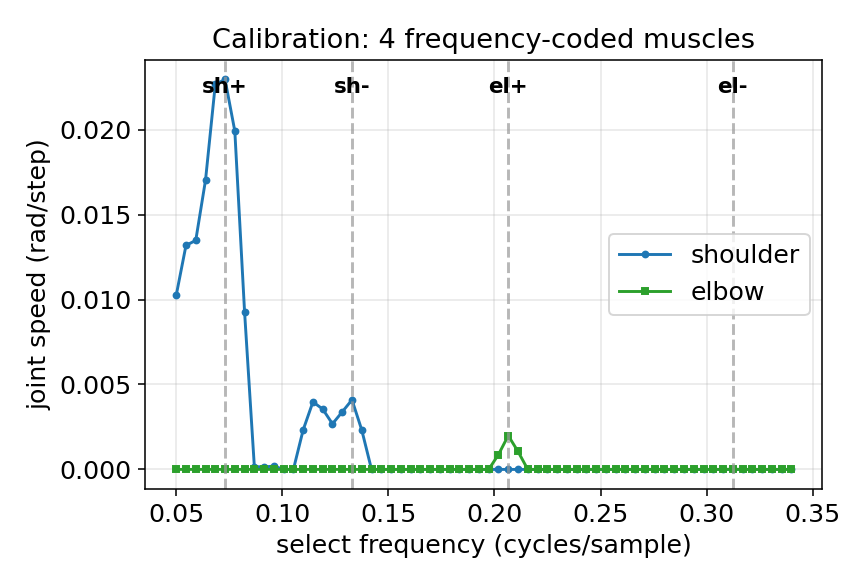
\includegraphics[width=0.95\linewidth]{calibration.png}
\caption{Offline calibration. Sweeping the select frequency and measuring the
steady joint angular velocity reveals four band-pass muscle peaks --- two per
joint --- giving the brain-invariant (frequency $\to$ joint, direction) map. The
peaks at higher frequency are weaker, the first signature of the low-pass brain.}
\label{fig:calib}
\end{figure}

\section{Experimental design and evaluation methodology}
\label{sec:method}
All controllers are evaluated through the group-standard harness so that numbers
are commensurable: an identical polar grid of targets (radii
$\{20,38,55\}$\,cm $\times$ 8 angles), a fixed brain seed, a fixed horizon
($T=1000$), and the same six metrics. The grid spans the full reachable workspace
rather than a few hand-picked points, which is essential here because the failure
is \emph{directionally structured} and a few targets would hide it. The six
metrics are chosen to expose distinct aspects: \emph{final distance} (the headline
task error), \emph{time-to-threshold} (responsiveness), \emph{steady-state
distance} (settling/precision), \emph{shoulder and elbow angle error} (a
diagnostic decomposition that localises the failure), \emph{control effort}
(efficiency, and a guard against input saturation), and a \emph{spatial heatmap}
of final error (the structure of success and failure). Because the plant is
stochastic and brains vary, robustness is examined separately by re-running across
seeds and by perturbing the controller's own parameters.

\begin{figure}[t]
\centering
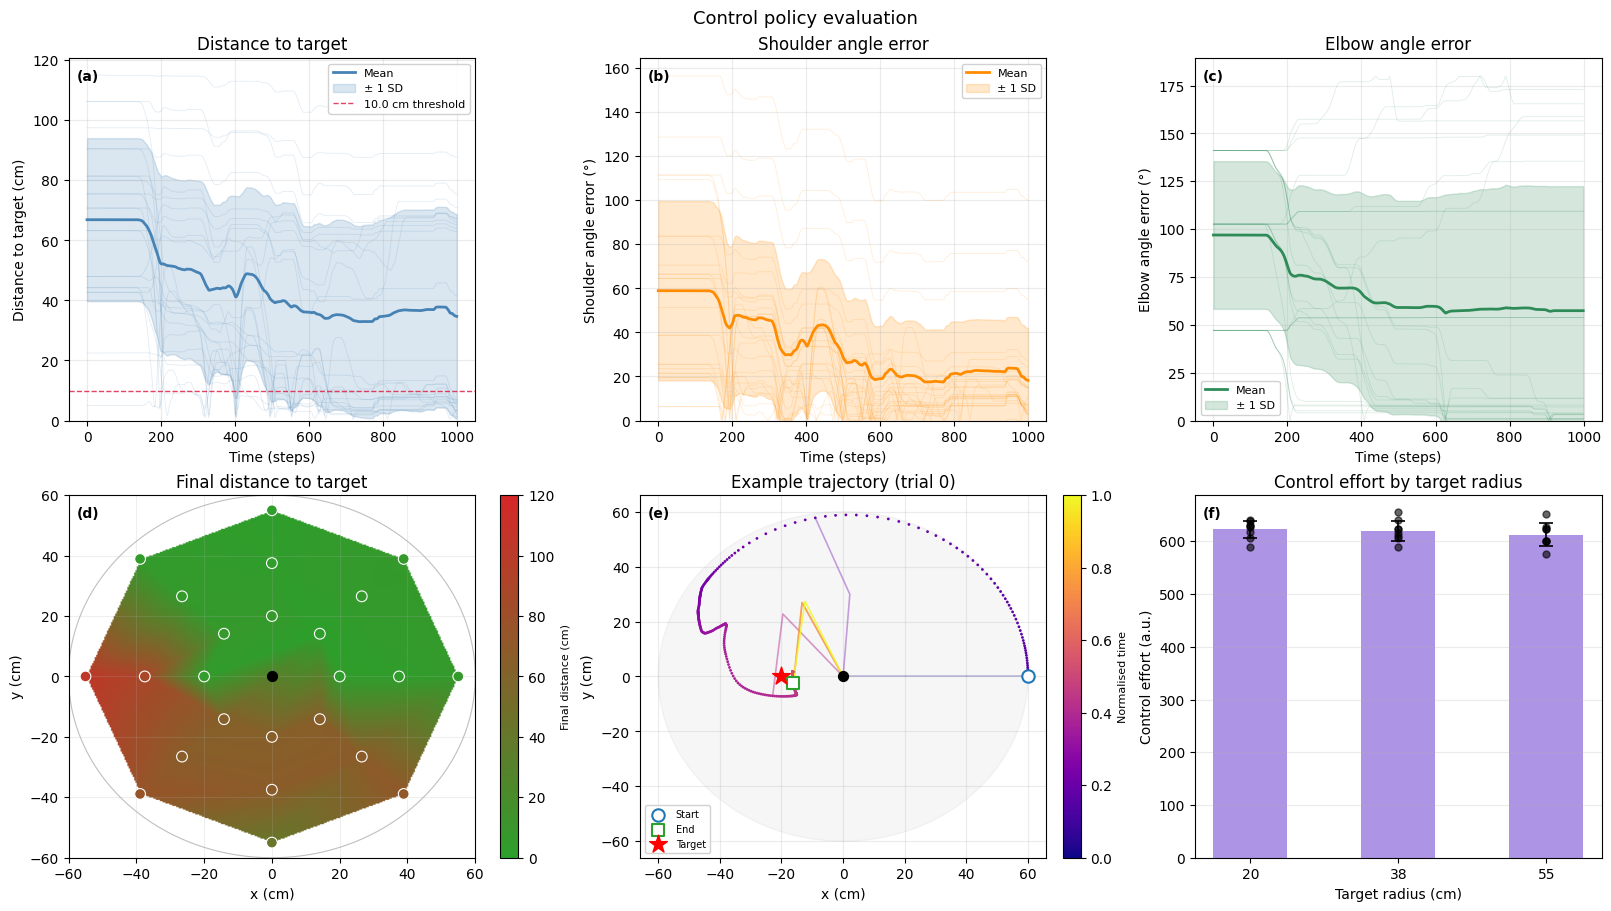
\includegraphics[width=0.9\textwidth]{template_eval.png}
\caption{Standardised evaluation on the polar target grid (seed 0, $T=1000$).
(a) Distance-to-target: a $\sim$150-step power ramp, then a plateau with a wide
band --- the signature of a bimodal outcome. (b,c) Shoulder vs.\ elbow angle
error: the shoulder error falls but the \emph{elbow} error stays high, localising
the bottleneck. (d) Final-distance heatmap: the failure is sharply
\emph{directional} --- a reachable upper/right region (green, $\le12$\,cm) and a
red lower/far-left shortfall ($53$--$103$\,cm). (e) Example trajectory: the hand
sweeps over the top and curls in. (f) Effort is flat across radius, so the failing
targets spend effort without converging --- an actuation limit, not under-driving.}
\label{fig:eval}
\end{figure}

\section{Results and performance analysis}
\label{sec:results}
\paragraph{Aggregate performance.} On the official grid (Fig.~\ref{fig:eval}) the
final distance is $32.3\pm33.4$\,cm, the shoulder error $19.3\pm23.1^\circ$, and
the elbow error $53.1\pm63.0^\circ$, with time-to-threshold $401\pm211$ steps and
near-constant control effort ($617\pm23$). In every metric the standard deviation
is comparable to the mean: the average hides a sharply \emph{bimodal} outcome.

\paragraph{A directionally-structured failure.} Splitting the grid by workspace
half makes the bimodality explicit:

\begin{center}
\small
\begin{tabular}{lccc}
\toprule
half & final dist.\ & $|$shoulder err$|$ & $|$elbow err$|$ \\
\midrule
upper ($y>0$) & $5.7$\,cm & $7^\circ$ & $7^\circ$ \\
lower ($y<0$) & $61.6$\,cm & $47^\circ$ & $101^\circ$ \\
\bottomrule
\end{tabular}
\end{center}

The upper half is reached to a few centimetres; the lower half misses by $\sim
60$\,cm, and the residual is overwhelmingly elbow error. The cause is the low-pass
brain (\S\ref{sec:plant}): the two halves recruit different members of each
antagonist pair. Measured joint authority falls monotonically with frequency ---
shoulder$+$ ($0.073$) gives $9.7$\,rad of travel, shoulder$-$ ($0.133$) $2.0$,
elbow$+$ ($0.207$) $2.0$, elbow$-$ ($0.312$) only $0.9$. The upper half uses the
strong, low-frequency muscles; the lower half needs the weak, high-frequency ones,
above all the near-dead elbow$-$, which cannot bend the elbow the required way.
That the control effort is flat across radius (Fig.~\ref{fig:eval}f) confirms this
is an \emph{actuation} limit: the failing targets expend effort without
converging, so more stimulation would not help.

\paragraph{Generalisation across brains.} Calibration is performed once but every
trial is a different random brain. Across five seeds on a common target set the
controller reaches a median of $10.2$\,cm with $93\%$ of trials within $15$\,cm:
the brain-invariant structure transfers, and the loop absorbs each brain's gain.

\paragraph{Value of feedback (V1 vs.\ V2).} Sharing the entire servo and differing
only in the joint estimate, V1 (hand feedback) reaches a median $10.2$\,cm while
V2 (neural observer, no hand feedback) reaches $33.7$\,cm with $0\%$ within
$15$\,cm. The observer runs correctly but drifts on the $\sim$10$\times$ noisier
single-sample neural; the $\sim$24\,cm gap quantifies the worth of direct hand
sensing under this plant's noise.

\paragraph{Parameter sensitivity, and a cautionary result.} On the calibration
brain alone, raising the elbow gain improves accuracy, suggesting an easy win.
\emph{Cross-seed validation overturns this}: reliability (within 15\,cm) \emph{falls}
from $90\%$ at the default boost to $65\%$ at a larger one, because over-driving
the elbow on brains where it is adequate induces overshoot. The single-seed gain
was over-fitting. This is itself a methodological finding --- on a stochastic,
per-brain-varying plant, single-brain tuning is misleading and parameters must be
chosen by cross-seed reliability. The deadzone tolerance, by contrast, is nearly
inert, showing the loop is not delicate.

\section{Strengths, limitations and alternatives}
\paragraph{Strengths.} The controller is simple, requires no online model
inversion, generalises across brains, and exploits rather than fights the
decoder's structure (frequency selection plus free power). Its failure is
interpretable and localised to a single physical cause.

\paragraph{Limitations.} (i) \emph{Elbow under-actuation} dominates: the
higher-frequency muscles are low-pass-attenuated, so interior/lower targets are
reach-limited (the directional failure above). (ii) \emph{Shared input budget}:
two simultaneous tones split the $[0,1]$ amplitude, starving the weak elbow most.
(iii) \emph{Overshoot}: the head's slow power ramp and fast exit make the smallest
effective stimulation larger than the final correction, so the hand hunts near the
target rather than settling. (iv) \emph{Dependence on hand sensing}: without it,
V2 drifts (10$\to$34\,cm). (v) \emph{Stochastic stalls} from measurement noise,
recovered by feedback at a cost in time.

\paragraph{Comparison with alternatives.} The rejected model-based strategies
(LQG, Fourier inversion, MPC) each fail a hard requirement --- closing the loop on
the hand and/or crossing the nonlinearity without a full model --- whereas the
select-tone servo does both by using the head's structure. Within the group, the
sharpest contrast is with a \emph{time-domain primitive finite-state-machine}
controller: it rests on the \emph{same} four rhythmic primitives but drives them
as discrete, FSM-supervised bursts rather than continuous amplitude-proportional
tones. Strikingly, the two structurally different controllers converge on the
\emph{same} precision wall --- the minimum effective stimulation exceeds the fine
correction. This is strong evidence that the binding limit is a property of the
\emph{plant} (the power ramp/exit asymmetry and stiction granularity), not of
either control law, and is the most important cross-approach lesson.

\section{Future improvements and conclusion}
Three improvements follow directly from the analysis. First, \emph{IK-branch
selection by muscle strength}: most targets admit two arm configurations
(elbow-up/down); the controller currently takes the one nearest the home pose,
which for the lower half forces the weak elbow$-$. Choosing the branch that
recruits the strong, low-frequency muscles would, in software alone, turn much of
the red lower half green --- and the example trajectory (Fig.~\ref{fig:eval}e),
which reaches a lower target by sweeping over the top with the strong muscle, shows
this already works when geometry permits. Second, a \emph{per-trial elbow
self-calibration} rather than a fixed gain that over-fits one brain. Third,
\emph{sub-primitive actuation} --- graded micro-bursts or amplitude annealing on
approach --- to beat the overshoot wall that no high-level controller removes.

In summary, exploiting the decoder as a frequency-addressed muscle bank with free
power yields a controller that is simple, generalises across brains, and localises
its failure to one physical bottleneck: the weak, high-frequency elbow muscles of
a low-pass brain. The work also yields two transferable lessons --- that direct
hand sensing is worth $\sim$24\,cm here, and that on a stochastic, varying plant,
rigorous evaluation must be cross-seed, because best-case tuning misleads.

\end{document}
